
\documentclass[tikz,border=3mm]{standalone}
\usepackage{tikz}
\usetikzlibrary{positioning,arrows.meta,calc}
\begin{document}
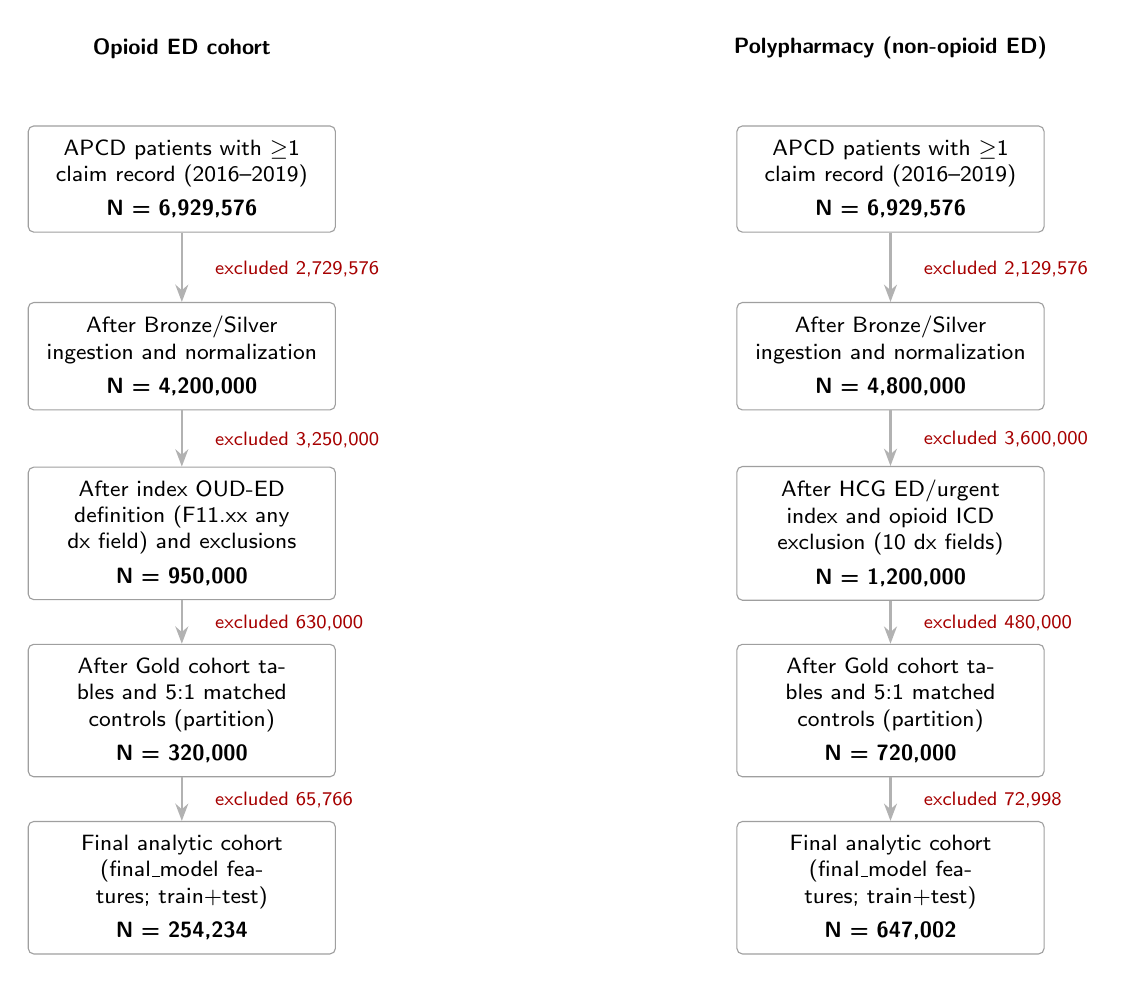
\begin{tikzpicture}[
  font=\footnotesize\sffamily,
  box/.style={draw, rounded corners=2pt, align=center, text width=3.55cm,
    minimum height=1.05cm, inner sep=5pt, fill=white, draw=gray!75},
  arr/.style={-{Stealth[length=2.2mm]}, thick, draw=gray!60},
  excl/.style={font=\scriptsize\sffamily, text=red!65!black},
  every node/.style={align=center}
]
\node[font=\bfseries\footnotesize\sffamily, anchor=south] (hdr-opioid) at (0.00,0.35) {Opioid ED cohort};
\node[box] (box-opioid-0) at (0.00,-1.05) {APCD patients with $\geq$1 claim record (2016--2019) \\[0.35em] \textbf{N = 6,929,576}};
\node[box] (box-opioid-1) at (0.00,-3.30) {After Bronze/Silver ingestion and normalization \\[0.35em] \textbf{N = 4,200,000}};
\node[box] (box-opioid-2) at (0.00,-5.55) {After index OUD-ED definition (F11.xx any dx field) and exclusions \\[0.35em] \textbf{N = 950,000}};
\node[box] (box-opioid-3) at (0.00,-7.80) {After Gold cohort tables and 5:1 matched controls (partition) \\[0.35em] \textbf{N = 320,000}};
\node[box] (box-opioid-4) at (0.00,-10.05) {Final analytic cohort (final\_model features; train+test) \\[0.35em] \textbf{N = 254,234}};
\path (box-opioid-0.south) -- (box-opioid-1.north) coordinate[pos=0.52] (mid-opioid-1);
\node[excl, anchor=west] at ([xshift=3mm]mid-opioid-1) {excluded 2,729,576};
\path (box-opioid-1.south) -- (box-opioid-2.north) coordinate[pos=0.52] (mid-opioid-2);
\node[excl, anchor=west] at ([xshift=3mm]mid-opioid-2) {excluded 3,250,000};
\path (box-opioid-2.south) -- (box-opioid-3.north) coordinate[pos=0.52] (mid-opioid-3);
\node[excl, anchor=west] at ([xshift=3mm]mid-opioid-3) {excluded 630,000};
\path (box-opioid-3.south) -- (box-opioid-4.north) coordinate[pos=0.52] (mid-opioid-4);
\node[excl, anchor=west] at ([xshift=3mm]mid-opioid-4) {excluded 65,766};
\draw[arr] (box-opioid-0.south) -- (box-opioid-1.north);
\draw[arr] (box-opioid-1.south) -- (box-opioid-2.north);
\draw[arr] (box-opioid-2.south) -- (box-opioid-3.north);
\draw[arr] (box-opioid-3.south) -- (box-opioid-4.north);
\node[font=\bfseries\footnotesize\sffamily, anchor=south] (hdr-polypharmacy) at (9.00,0.35) {Polypharmacy (non-opioid ED)};
\node[box] (box-polypharmacy-0) at (9.00,-1.05) {APCD patients with $\geq$1 claim record (2016--2019) \\[0.35em] \textbf{N = 6,929,576}};
\node[box] (box-polypharmacy-1) at (9.00,-3.30) {After Bronze/Silver ingestion and normalization \\[0.35em] \textbf{N = 4,800,000}};
\node[box] (box-polypharmacy-2) at (9.00,-5.55) {After HCG ED/urgent index and opioid ICD exclusion (10 dx fields) \\[0.35em] \textbf{N = 1,200,000}};
\node[box] (box-polypharmacy-3) at (9.00,-7.80) {After Gold cohort tables and 5:1 matched controls (partition) \\[0.35em] \textbf{N = 720,000}};
\node[box] (box-polypharmacy-4) at (9.00,-10.05) {Final analytic cohort (final\_model features; train+test) \\[0.35em] \textbf{N = 647,002}};
\path (box-polypharmacy-0.south) -- (box-polypharmacy-1.north) coordinate[pos=0.52] (mid-polypharmacy-1);
\node[excl, anchor=west] at ([xshift=3mm]mid-polypharmacy-1) {excluded 2,129,576};
\path (box-polypharmacy-1.south) -- (box-polypharmacy-2.north) coordinate[pos=0.52] (mid-polypharmacy-2);
\node[excl, anchor=west] at ([xshift=3mm]mid-polypharmacy-2) {excluded 3,600,000};
\path (box-polypharmacy-2.south) -- (box-polypharmacy-3.north) coordinate[pos=0.52] (mid-polypharmacy-3);
\node[excl, anchor=west] at ([xshift=3mm]mid-polypharmacy-3) {excluded 480,000};
\path (box-polypharmacy-3.south) -- (box-polypharmacy-4.north) coordinate[pos=0.52] (mid-polypharmacy-4);
\node[excl, anchor=west] at ([xshift=3mm]mid-polypharmacy-4) {excluded 72,998};
\draw[arr] (box-polypharmacy-0.south) -- (box-polypharmacy-1.north);
\draw[arr] (box-polypharmacy-1.south) -- (box-polypharmacy-2.north);
\draw[arr] (box-polypharmacy-2.south) -- (box-polypharmacy-3.north);
\draw[arr] (box-polypharmacy-3.south) -- (box-polypharmacy-4.north);
\end{tikzpicture}
\end{document}
